
\begin{frame}
    % \small
    % \begin{PointSix}{How do we teach? }
    %     \begin{itemize}
    %         \item Video Lectures or Plenum (Tuesdays)
    %         \item Exercises \& 1-1-Interaction (Thursdays)
    %         \item Applied Exercises (Magnetics, Electrics, Seismics)
    %     \end{itemize}
    % \end{PointSix}
\end{frame}

\begin{frame}
  \begin{PointSix}{Introduction}
    \small
    \alert{Introduction to Geophysics}
    \begin{itemize}
      \item Who?
      \item What?
      \item How?
    \end{itemize}
  \end{PointSix}
  \end{frame}

\begin{frame}
    \begin{PointSix}{Who's teaching?}
        \small
        \begin{itemize}
            \item R. Drews (Prof. Geophysics at UT)
            \item P. Dietrich (Prof. Env./Eng.- Geophysics at UFZ, Leipzig)
            \item R. Ershadi (PhD Geophysics)
            \item A. Vinson (TA, MSc Geosciences)
            \item L. Naumann (TA, BSc Geosciences)
          \end{itemize}
    \end{PointSix}
\end{frame}

\begin{frame}
    \begin{PointSix}{Who's teaching?}
        \alert{Introduction to Geophysics - R. Drews}
        \small Prof. for Geophysics since 2022
      \end{PointSix}
\end{frame}

\begin{frame}
    \begin{PointSix}{Who's teaching?}
        \alert{Introduction to Geophysics - R. Drews}
        \small Prof. for Geophysics since 2022
        \includegraphics[width=0.99\textwidth]{Figures/General/FieldPhotos/GPRColle.png}
      \end{PointSix}
\end{frame}

\begin{frame}
    \begin{PointSix}{Who's teaching?}
        \alert{Introduction to Geophysics - R. Drews}
        \small Prof. for Geophysics since 2022
        \includegraphics[width=0.99\textwidth]{Figures/General/FieldPhotos/GPRColle2.png}
      \end{PointSix}
\end{frame}

\begin{frame}
    \begin{PointSix}{Who's teaching?}
        \alert{Introduction to Geophysics - R. Drews}
        \small Prof. for Geophysics since 2022
        \includegraphics[width=0.99\textwidth]{Figures/General/FieldPhotos/PriestleyHelicopter.JPG}
      \end{PointSix}
\end{frame}

\begin{frame}
    \begin{PointSix}{Who's teaching?}
        \alert{Introduction to Geophysics - R. Drews}
        \small Prof. for Geophysics since 2022
        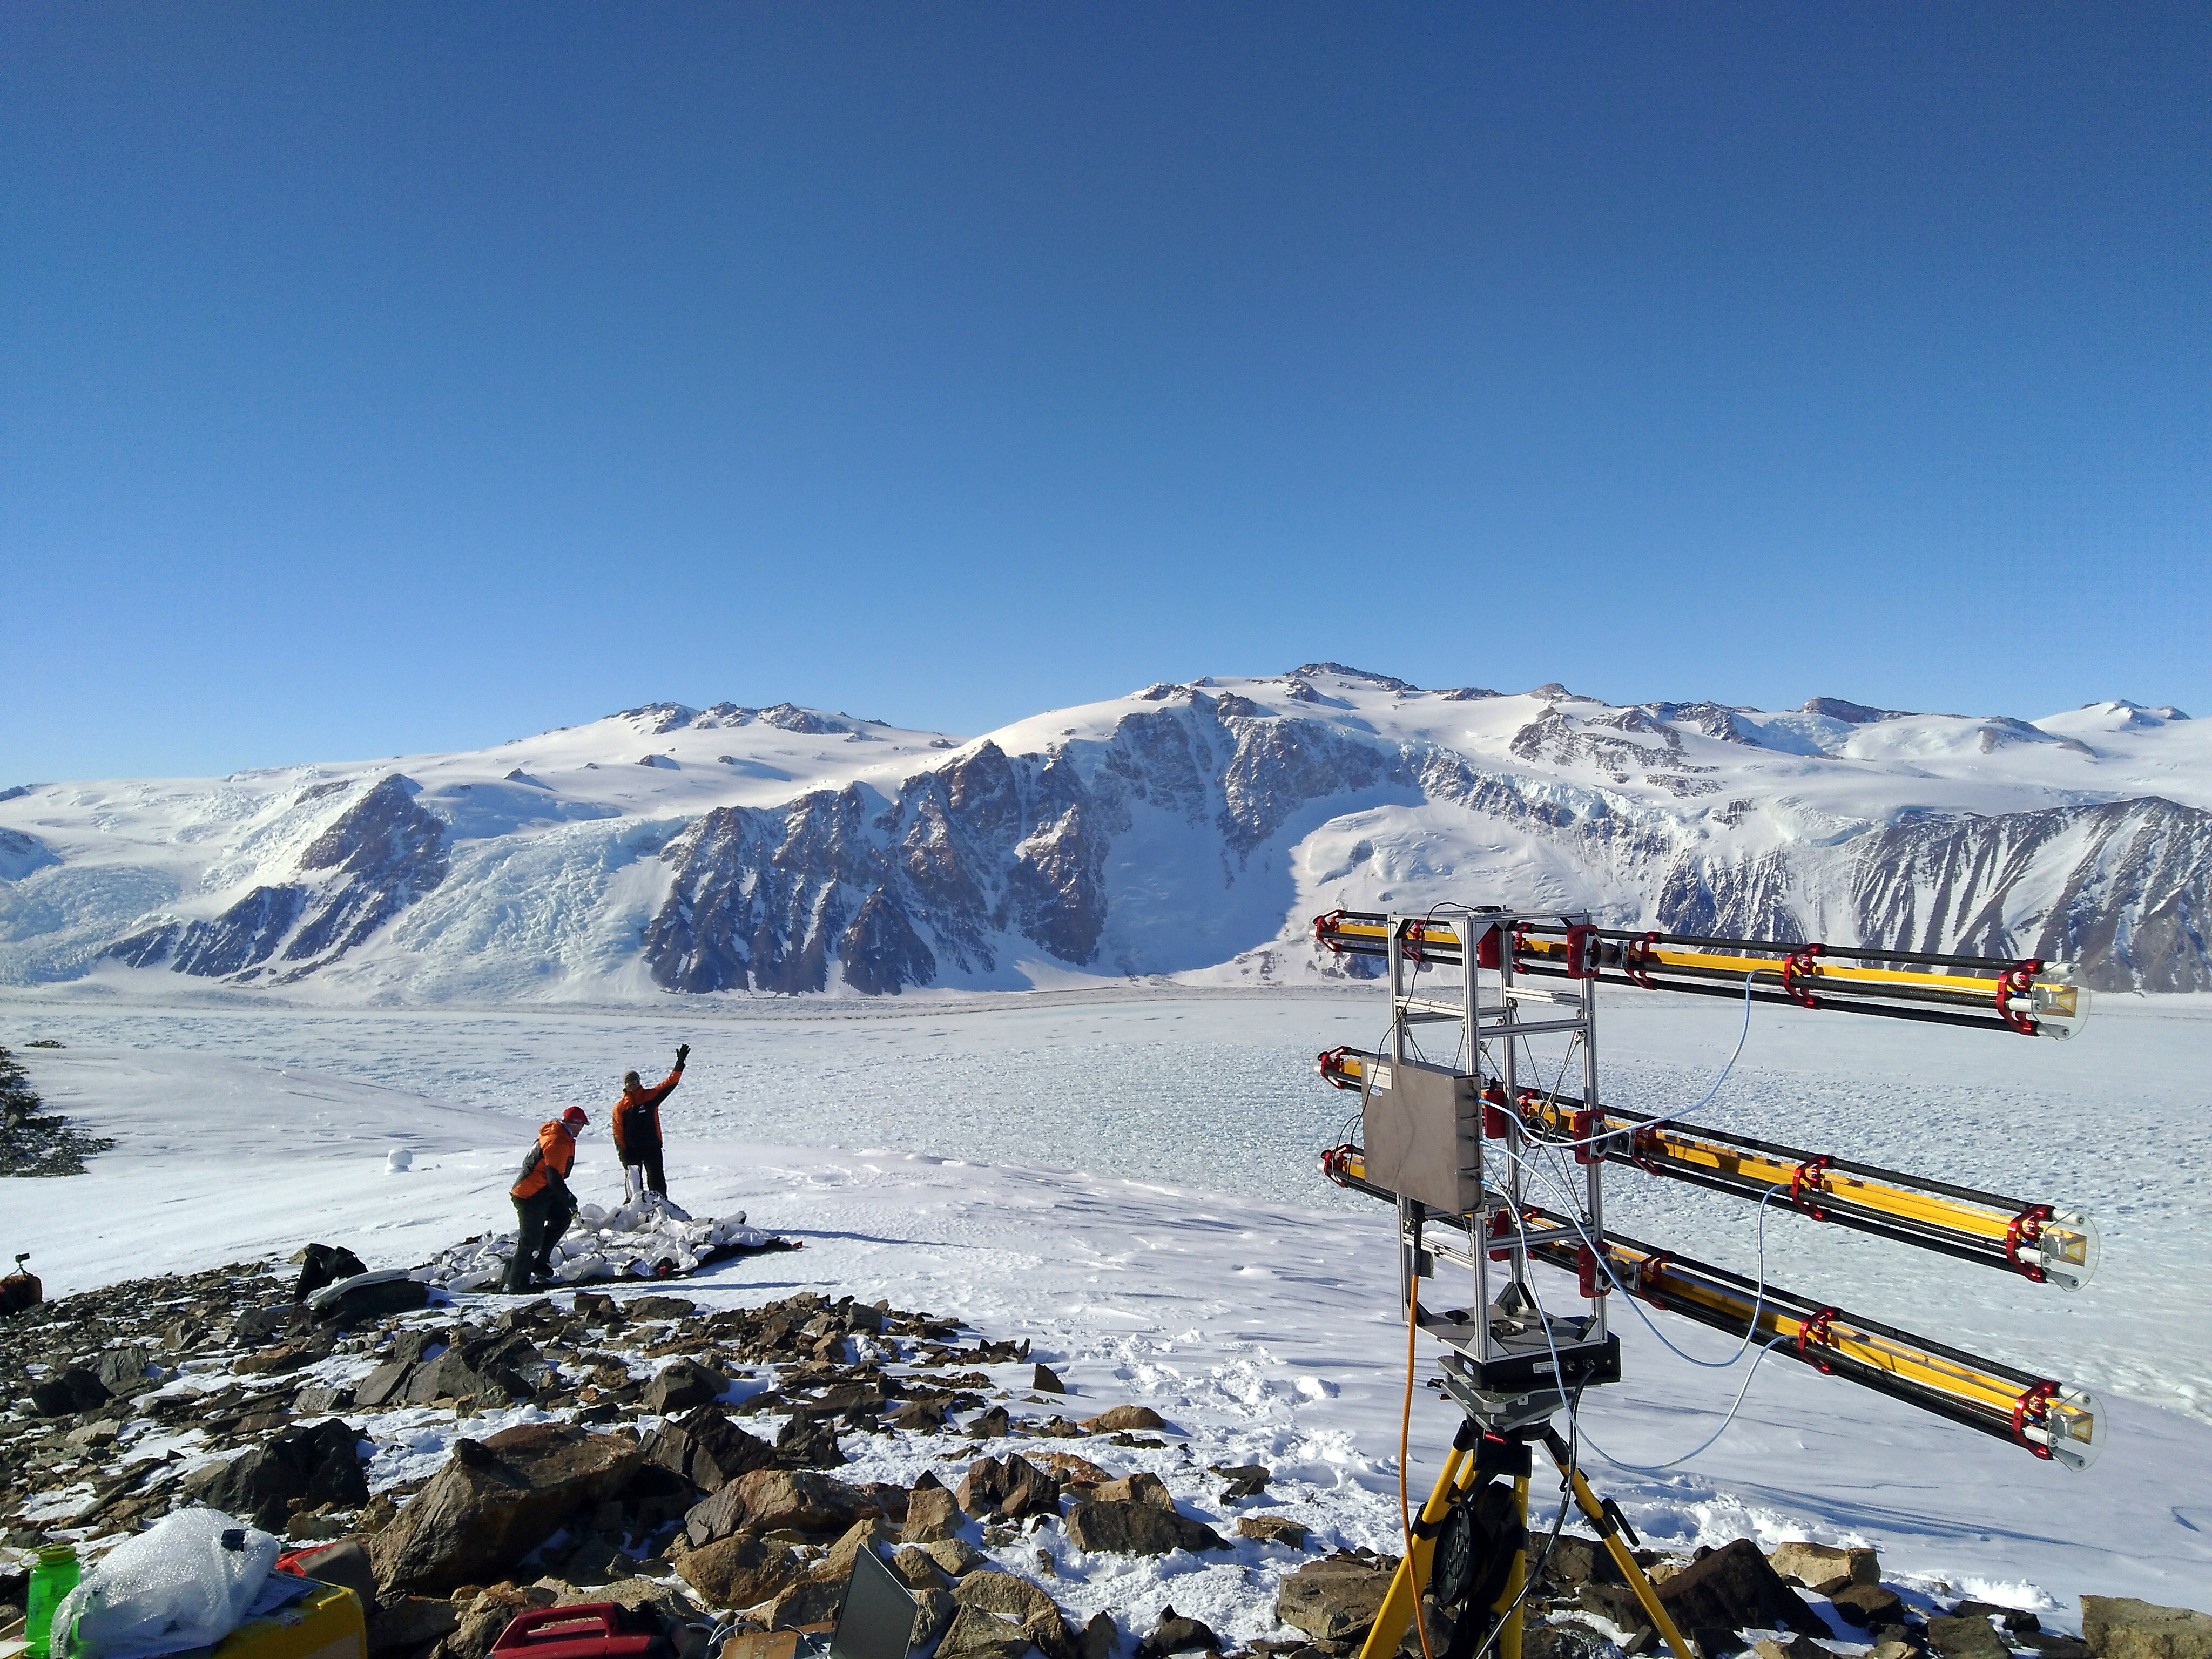
\includegraphics[width=0.99\textwidth]{Figures/General/FieldPhotos/GPRI.jpg}
      \end{PointSix}
\end{frame}

\begin{frame}
    \begin{PointSix}{Who's teaching?}
        \alert{Introduction to Geophysics - R. Drews}
        \small Prof. for Geophysics since 2022
        \includegraphics[width=0.99\textwidth]{Figures/General/FieldPhotos/ApenninsGPR.jpg}
      \end{PointSix}
\end{frame}


\begin{frame}
    \begin{PointSix}{What are we teaching?}
        \small
        \alert{Geophysics} is a branch of earth science dealing with the physical processes and phenomena occurring especially in the earth and in its vicinity.\\
        \vspace{0.25cm}
        \tiny [Merriam-Webster]\\
        \small
        \vspace{2.25cm}
        \alert{Applied Geophysics} is a branch of Geophysics dealing with different observational methods imaging the sub-surface.\\
        \vspace{0.25cm}
        \tiny [The lecture focus will be here.]
    \end{PointSix}
\end{frame}

\begin{frame}
    \begin{PointSix}{What are we teaching?}
        \small
        \alert{Applied Geophysics} contains, e.g, gravity, magnetics, electrics, electrical induction, electromagnetics (radar), seismics.\\
        \vspace{0.25cm}
        \tiny [Focus on physical principals rather than aquisition specifics.]
    \end{PointSix}
\end{frame}

\begin{frame}
    \begin{PointSix}{Example: Seismics}
        \includegraphics[width=0.99\textwidth]{Figures/General/GeophysExamples/Seismics_SvdLEE_Evanston_IL.png}
        \tiny[S. van der Lee, Northwestern University, Evanston, IL]
        %Data gathered by a network of seismic instruments (red) have enabled researchers to discern a region of relatively cold, stiff rock (shades of green and blue) beneath eastern North America. This is likely to be the remnants of an ancient tectonic plate. Image credit: Suzan van der Lee (Northwestern University, Evanston, IL).

    \end{PointSix}
\end{frame}

\begin{frame}
    \begin{PointSix}{Example: Magnetics}
        \includegraphics[width=0.99\textwidth]{Figures/General/GeophysExamples/Magnetics1_FassbinderBADS.png}
        \tiny[Fassbinder, Bavarian Academy of Sciences]
           \end{PointSix}
\end{frame}
\begin{frame}
    \begin{PointSix}{Example: Magnetics}
        \includegraphics[width=0.99\textwidth]{Figures/General/GeophysExamples/Magnetics2_FassbinderBADS.png}
        \tiny[Fassbinder, Bavarian Academy of Sciences]
           \end{PointSix}
\end{frame}
\begin{frame}
    \begin{PointSix}{Example: Geoelectrics}
        \includegraphics[width=0.9\textwidth]{Figures/General/GeophysExamples/DCElectricsSinkhole_Plank2019NearSurfaceGeophys_Reversed.png}

        \tiny[Plank et al., Near Surface Geophysics, 2019]
        %Volumetric interpretation of the former sinkhole at 900 Ωm isovalue. The resistivity scale is not artificially distorted. The yellow lines indicate the traces of 2D geoelectric survey lines. The crossing point is not above the sinkhole.
        \end{PointSix}
\end{frame}

\begin{frame}
    \begin{PointSix}{Example: Gravity}
        \includegraphics[width=0.90\textwidth]{Figures/Gravity/Exported/Grace_JPLCaltect_FODT10_WithoutPeople.png}
    \end{PointSix}
\end{frame}



\begin{frame}
    \small
    \begin{PointSix}{How do we teach? }
        \begin{itemize}
            \item Video Lectures or Plenum (Tuesdays)
            \item Exercises \& 1-1-Interaction (Thursdays)
            \item Applied Exercises (Magnetics, Electrics, Seismics)
        \end{itemize}
    \end{PointSix}
\end{frame}

\begin{frame}
    \begin{PointSix}{How do we teach?}
        \small
        \alert{Learning Goals}
        \begin{itemize}
            \item Obtain a broad overview of geophysical methods for sub-surface imaging.
            \item Understand the underlying physical principles.
            \item Learn how to think logically \& quantitatively.
        \end{itemize}
    \end{PointSix}
\end{frame}

\begin{frame}
    \begin{PointThree}{How do we teach?}
        \small
        \alert{Expectations}
        \begin{itemize}
            \item Be prepared.
            \item Ask questions.
            \item Do the work.
        \end{itemize}
    \end{PointThree}
\end{frame}

\begin{frame}
    \begin{PointSix}{How do we teach? $\rightarrow$ Ilias}
        \includegraphics[width=0.90\textwidth]{Figures/General/LectureOutline_PageOne.jpg}
    \end{PointSix}
\end{frame}